\documentclass{MO}

\author{Dominik Dembinný}
\studentclass{2. F / 4 Gymnázium}
\school{Arabská 14, Praha 6}

\usetikzlibrary{calc, intersections, through, angles, quotes}
\usepackage{amsmath, amssymb, amsthm}

\problemcategory{75}{B}{I}{4}


\begin{document}
\makeMOheader

\section*{Problem Statement}
In a convex quadrilateral $ABCD$, it holds that $|\angle ABC| = |\angle ADC|$ and $|\angle BCD| = 3|\angle BAD|$. Points $P$ and $Q$ lie on segments $AB$ and $AD$ respectively, such that $APCQ$ is a parallelogram. Let $O$ be the circumcenter of triangle $CPQ$. Prove that $AO \perp BD$.

\section*{Proof}

\subsection*{Step 1: Angle Analysis}
Let $\alpha = |\angle BAD|$.
Given that $|\angle BCD| = 3\alpha$ and the sum of angles in a quadrilateral is $360^\circ$, we have:
\[
    \alpha + |\angle ABC| + 3\alpha + |\angle ADC| = 360^\circ
\]
Since $|\angle ABC| = |\angle ADC|$, let us denote their measure by $\beta$. The equation becomes:
\[
    4\alpha + 2\beta = 360^\circ \implies 2\alpha + \beta = 180^\circ \implies \beta = 180^\circ - 2\alpha
\]
Thus, angles $\angle ABC$ and $\angle ADC$ are supplementary to $2\alpha$.

\subsection*{Step 2: Properties of Triangles $PBC$ and $QDC$}
Since $APCQ$ is a parallelogram, we have $PC \parallel AD$ and $CQ \parallel AB$. Also, opposite angles of the parallelogram are equal: $|\angle PCQ| = |\angle PAQ| = \alpha$.

Consider $\triangle PBC$:
\begin{itemize}
    \item The angle at vertex $B$ is $\beta = 180^\circ - 2\alpha$.
    \item Since $PC \parallel AD$ and $AB$ intersects them, $\angle BPC$ corresponds to $\angle DAB$, so $|\angle BPC| = \alpha$.
    \item The remaining angle is $|\angle BCP| = 180^\circ - (180^\circ - 2\alpha) - \alpha = \alpha$.
\end{itemize}
Since $|\angle BCP| = |\angle BPC| = \alpha$, $\triangle PBC$ is isosceles with $\mathbf{PB = BC}$.

Similarly for $\triangle QDC$:
\begin{itemize}
    \item The angle at vertex $D$ is $\beta = 180^\circ - 2\alpha$.
    \item Since $CQ \parallel AB$ and $AD$ intersects them, $|\angle DQC| = \alpha$.
    \item The remaining angle is $|\angle QCD| = \alpha$.
\end{itemize}
Thus, $\triangle QDC$ is isosceles with $\mathbf{QD = DC}$.

\subsection*{Step 3: Characterizing Point $O$}
Point $O$ is the circumcenter of $\triangle CPQ$, so it satisfies $|OC| = |OP| = |OQ|$.
\begin{itemize}
    \item Since $|OP| = |OC|$ and $|BP| = |BC|$, both $O$ and $B$ lie on the perpendicular bisector of segment $PC$. Therefore, $BO \perp PC$.
    \item Since $|OQ| = |OC|$ and $|DQ| = |DC|$, both $O$ and $D$ lie on the perpendicular bisector of segment $QC$. Therefore, $DO \perp QC$.
\end{itemize}

\subsection*{Step 4: Orthocenter of $\triangle ABD$}
We utilize the parallel properties of the parallelogram $APCQ$:
\begin{enumerate}
    \item We established $BO \perp PC$. Since $PC \parallel AD$, it follows that $\mathbf{BO \perp AD}$. (Line $BO$ contains the altitude from $B$ to $AD$).
    \item We established $DO \perp QC$. Since $QC \parallel AB$, it follows that $\mathbf{DO \perp AB}$. (Line $DO$ contains the altitude from $D$ to $AB$).
\end{enumerate}
Since $O$ is the intersection of these two altitudes, $O$ is the \textbf{orthocenter} of $\triangle ABD$.

\subsection*{Conclusion}
Since $O$ is the orthocenter of $\triangle ABD$, the line segment connecting the third vertex $A$ to $O$ must lie on the third altitude of the triangle. Consequently, this altitude is perpendicular to the opposite side $BD$.
\[
    AO \perp BD
\]
\hfill \qedsymbol

\newpage
\section*{Visualization}

\begin{center}
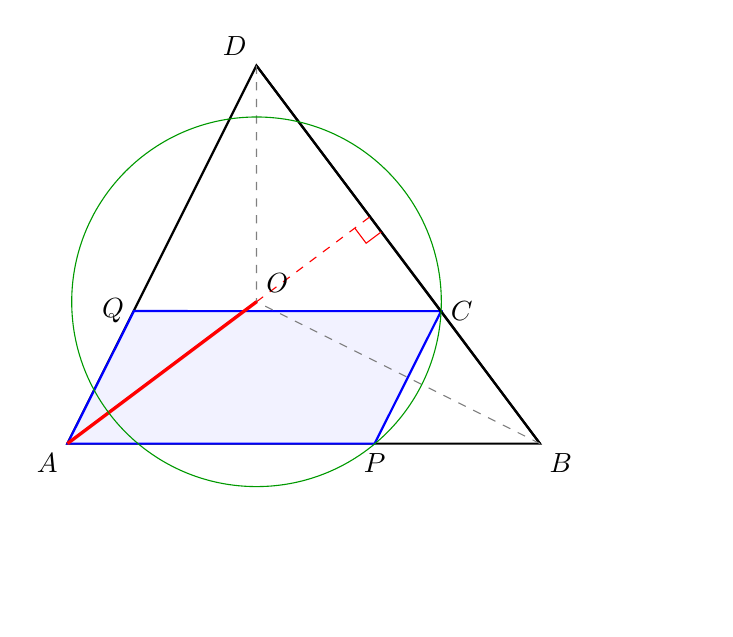
\begin{tikzpicture}[scale=1.2]
    % 1. Define Coordinates for Triangle ABD
    \coordinate (A) at (0,0);
    \coordinate (B) at (5,0);
    \coordinate (D) at (2, 4);

    % 2. Find Orthocenter O
    % Altitude from B to AD
    \coordinate (H_B) at ($(A)!(B)!(D)$); % Projection of B onto AD
    % Altitude from D to AB
    \coordinate (H_D) at (2,0); % Projection of D onto AB (since A is origin, B on x-axis)
    
    % Intersect altitudes to find O
    \path[name path=altB] (B) -- (H_B);
    \path[name path=altD] (D) -- (H_D);
    \path [name intersections={of=altB and altD, by=O}];

    % 3. Construct C based on logic:
    % P is on AB. Q is on AD.
    % PC || AD and QC || AB.
    % Also, O is circumcenter of CPQ.
    % Let's pick P on AB arbitrarily to satisfy diagram constraints.
    \coordinate (P) at ($(A)!0.65!(B)$); % P is 65% along AB
    
    % Line through P parallel to AD
    \path[name path=linePC] (P) -- ++($(D)-(A)$);
    
    % Line through O perpendicular to this line (bisector logic)
    % Wait, simpler construction based on P:
    % C must be such that APCQ is parallelogram.
    % So Q is on AD. Let's find Q.
    % Q is such that CQ || AB.
    % Let's find C by intersection of (Line P || AD) and (Line from Q || AB)? No Q is unknown.
    % Use: Vector AC = Vector AP + Vector AQ.
    % Use: C is reflection of P across bisector of angle A? No.
    % Use: PB = BC.
    % Circle centered at B passing through P.
    \node (B_node) at (B) {};
    \path[name path=circB] let \p1 = ($(B)-(P)$) in (B) circle ({veclen(\x1,\y1)});
    
    % Intersect Circle(B, BP) with Line(P || AD) to find C
    \path [name intersections={of=linePC and circB, by={C_sol}}];
    \coordinate (C) at (C_sol);
    
    % Define Q to complete parallelogram APCQ
    \coordinate (Q) at ($(A) + (C) - (P)$);
    
    % 4. Draw Geometry
    
    % Main Polygon ABCD
    \draw[thick] (A) -- (B) -- (C) -- (D) -- cycle;
    
    % Parallelogram APCQ
    \draw[blue, thick, fill=blue!5] (A) -- (P) -- (C) -- (Q) -- cycle;
    
    % Diagonal BD
    \draw[thick] (B) -- (D);
    
    % Altitudes / Lines to O
    \draw[dashed, gray] (B) -- (O); % Altitude to AD part
    \draw[dashed, gray] (D) -- (O); % Altitude to AB part
    
    % The Solution Line AO
    \draw[red, very thick] (A) -- (O);
    % Extend AO to BD to show perpendicularity
    \coordinate (H_A) at ($(B)!(A)!(D)$);
    \draw[red, dashed] (O) -- (H_A);
    
    % Circumcircle of CPQ (O is center)
    \draw[green!60!black, thin] (O) let \p1 = ($(O)-(C)$) in circle ({veclen(\x1,\y1)});

    % 5. Labels
    \node[below left] at (A) {$A$};
    \node[below right] at (B) {$B$};
    \node[right] at (C) {$C$};
    \node[above left] at (D) {$D$};
    \node[below] at (P) {$P$};
    \node[left] at (Q) {$Q$};
    \node[above right] at (O) {$O$};
    
    % Right Angle Mark at Intersection of AO and BD
    \draw[red] ($(H_A)!0.2cm!(A)$) -- ++($(H_A)!0.2cm!(B)-(H_A)$) -- ($(H_A)!0.2cm!(B)$);

\end{tikzpicture}
\end{center}

\end{document}